\documentclass{standalone}
\usepackage{tikz}
\usepackage{amsmath}
\usepackage{amsfonts}

% === TIPOGRAFÍA === (((
\usepackage{fontspec}
\setmainfont[
  BoldFont       = bodonibi,
	ItalicFont     = Century modern italic2.ttf,
	BoldItalicFont = bodonibi,
	SmallCapsFont  = lmromancaps10-regular.otf
]{Century_modern.ttf}
\DeclareSymbolFont{italics}{\encodingdefault}{\rmdefault}{m}{it}
\DeclareSymbolFontAlphabet{\mathit}{italics}
\ExplSyntaxOn
\int_step_inline:nnnn { `A } { 1 } { `Z }
 {  \exp_args:Nf \DeclareMathSymbol{\char_generate:nn{#1}{11}}{\mathalpha}{italics}{#1} }
\int_step_inline:nnnn { `a } { 1 } { `z } {  \exp_args:Nf \DeclareMathSymbol{\char_generate:nn{#1}{11}}{\mathalpha}{italics}{#1}}
\ExplSyntaxOff
% )))

\setlength{\fboxrule}{1.5pt}
\setlength{\fboxsep}{1.5pt}
\newcommand{\bloque}[1]{
	\rotatebox{90}{\fbox{\color{black} #1}}
}
\begin{document}

% \footnotesize 

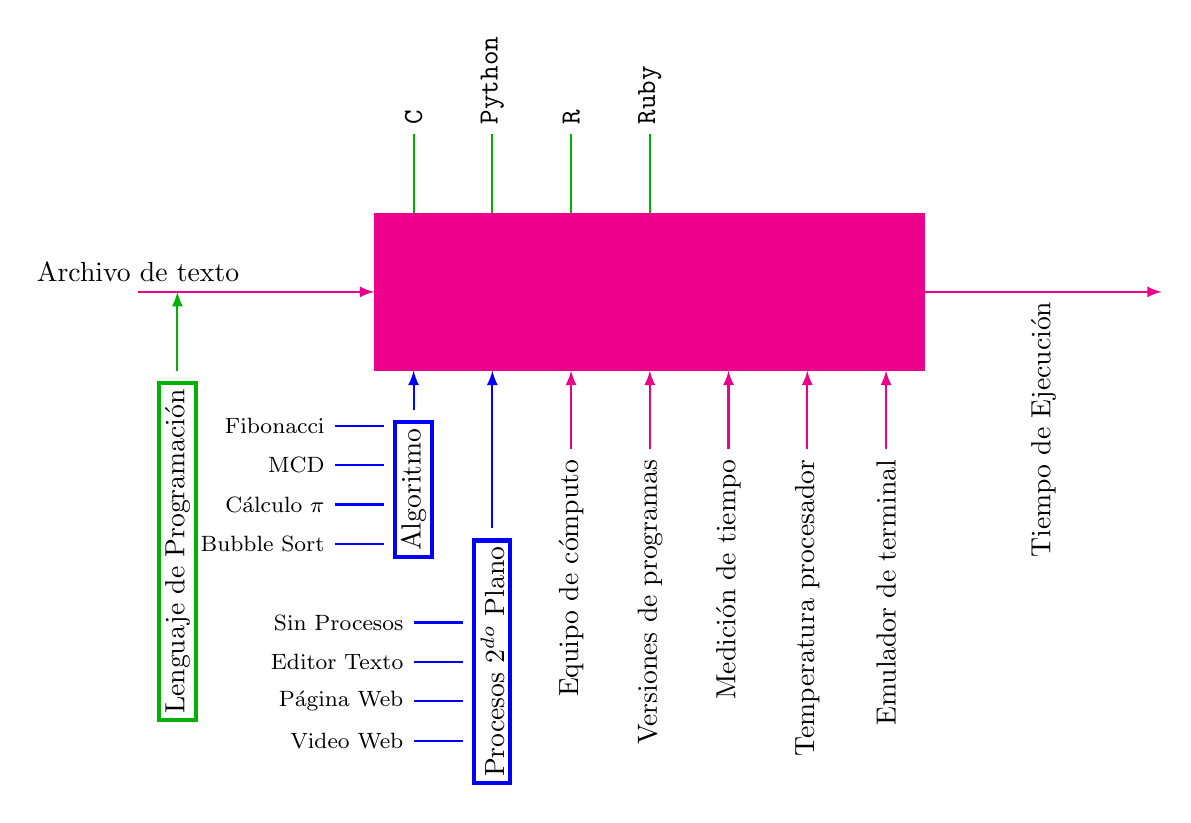
\begin{tikzpicture}[>=latex]
	\fill [magenta] (0,0) rectangle (7,2);
	\draw [thick , magenta , ->] (-3,1) node [black,above] {Archivo de texto} --++ (3,0);
	\draw [thick , magenta , ->] (7,1) --++ (3,0);
	\draw [thick , green!70!black,->] (-2.5,0) node [below] {\bloque{Lenguaje de Programación}} --++ (0,1);
	\begin{scope}[xshift=-0.5cm]
% FACTORES DE RUIDO
		\draw [blue, thick] (1,-0.7) --++ (-1,0) node [left] {\footnotesize \color{black} Fibonacci};
		\draw [blue, thick] (1,-1.2) --++ (-1,0) node [left] {\footnotesize \color{black} MCD};
		\draw [blue, thick] (1,-1.7) --++ (-1,0) node [left] {\footnotesize \color{black} Cálculo \(\pi\)};
		\draw [blue, thick] (1,-2.2) --++ (-1,0) node [left] {\footnotesize \color{black} Bubble Sort};
		\draw [thick ,blue,->] (1,-0.5) node [fill = white,below] {\bloque{Algoritmo}} --++ (0,0.5);
		\draw [blue, thick] (2,-3.2) --++ (-1,0) node [left] {\footnotesize \color{black} Sin Procesos};
		\draw [blue, thick] (2,-3.7) --++ (-1,0) node [left] {\footnotesize \color{black} Editor Texto};
		\draw [blue, thick] (2,-4.2) --++ (-1,0) node [left] {\footnotesize \color{black} Página Web};
		\draw [blue, thick] (2,-4.7) --++ (-1,0) node [left] {\footnotesize \color{black} Video Web};
		\draw [thick ,blue,->] (2,-2) node [fill = white,below] {\bloque{Procesos \(2^{do}\) Plano}} --++ (0,2);
		\draw [thick ,magenta,->] (3,-1) node [below] {\rotatebox{90}{\color{black} Equipo de cómputo}} --++ (0,1);
		\draw [thick ,magenta,->] (4,-1) node [below] {\rotatebox{90}{\color{black} Versiones de programas}} --++ (0,1);
		\draw [thick ,magenta,->] (5,-1) node [below] {\rotatebox{90}{\color{black} Medición de tiempo}} --++ (0,1);
		\draw [thick ,magenta,->] (6,-1) node [below] {\rotatebox{90}{\color{black} Temperatura procesador}} --++ (0,1);
		\draw [thick ,magenta,->] (7,-1) node [below] {\rotatebox{90}{\color{black} Emulador de terminal}} --++ (0,1);
% FACTORES CONTROLABLES
		\draw [thick , green!70!black] (1 ,2) --++ (0,1) node [above] {\rotatebox{90}{\color{black} \texttt{C}}};
		\draw [thick , green!70!black] (2 ,2) --++ (0,1) node [above] {\rotatebox{90}{\color{black} \texttt{Python}}};
		\draw [thick , green!70!black] (3 ,2) --++ (0,1) node [above] {\rotatebox{90}{\color{black} \texttt{R}}};
		\draw [thick , green!70!black] (4 ,2) --++ (0,1) node [above] {\rotatebox{90}{\color{black} \texttt{Ruby}}};
	\end{scope}
	\node [below] at (8.5,1) {\rotatebox{90}{Tiempo de Ejecución}};
\end{tikzpicture}

\end{document}
